\documentclass{article}

\usepackage{graphicx}
\usepackage{subcaption}

\title{Bone Cement Volumetry in sagittal and axial MRT-Images of the Spine}

\author{Friederici Anke, Jordan Grigori}

\begin{document}
  
  \maketitle
  \thispagestyle{empty}
  \pagebreak
  
  \section{Introduction}
  \setcounter{page}{1}
  {
  	We were introduced to the problem of semiautomatic bone cement volumetry 
  	on MR-images of a spline. The application to be developed is required 
  	to detect such regions of the spine reliably, which need to be treated with 
  	bone cement.\\
  	\\The data that is given presents the challenge, MR-images, which do not have
  	the strong contrast of CT-images nor are as noise free as CT-images, when it
  	comes to bone tissue. Thus more image processing becomes necessary to possibly 
  	achieve equally as good result as working with CT data.
  	At its core this is a non trivial segmentation task, which requires a thought 
  	through choice of image processing and segmentation algorithms.\\
  	\\Our approach was to split the solution to the problem in two steps:
  	\begin{enumerate}
  		\item Single out one vertebra of choice, by user input (e.g. a single mouse click).
  		\item Segment the chosen vertebra to its extent over the MR-images and measure the hollow regions volume, as precise as possible.
  	\end{enumerate}
  	We decided to keep it as simple as possible, by implementing the task at hand 
  	entirely on Matlab, by choosing an adequate segmentation algorithm called 
  	'Normalized Graph Cuts' \cite{[ShiMalik00]}, which only requires matrix operations.
  	\\Matlab also has its own implementation of an active contour
  	operation \cite{[ChanVese01]}, which could be used to segment the vertebra needed to a satisfying degree for the actual task of bone cement volumetry.\\	
  	\\In the following chapters we will first describe, how we implemented the vertebra segmentation.
  	After we will move on describing our chosen filling compound segmentation inside the vertebra.
  	At last in the remaining two chapters we will present our results and evaluate them, to see how well our application fare against the ground truth solution.
  }
  
  \section{Vertebra Segmentation}
  \begin{itemize}
  	\item Hi, I'm a bullet point!
  	\item $And~ I'm~ a~ F{\sigma}rmul{\alpha}! \sum_{bottom}^{top}$
  \end{itemize}
  
  \section{Filling Compound Segmentation}
  
  \section{Results}
  \begin{figure}[h]
          \centering
    \begin{subfigure}[t]{0.45\linewidth}
      \centering
      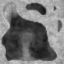
\includegraphics{test.png}
      \caption{Subfigures \textit{woopwoop}}
    \end{subfigure}
    \hfill
    \begin{subfigure}[t]{0.45\linewidth}
      \centering
      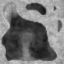
\includegraphics{test.png}
      \caption{Another really awesome image}
    \end{subfigure}
    \caption{These are some awesome images}
  \end{figure}
  
  \section{Evaluation}
  
  
	\begin{thebibliography}{9}
	
	\bibitem{[ChanVese01]}
	T. F. Chan and L. A. Vese,
	\emph{"Active contours without edges", IEEE Transactions on Image Processing},
	vol. 10, Issue 2, pp. 266-277, 2001.
	
	
	\bibitem{[ShiMalik00]}
	J.  Shi  and  J.  Malik,
	\emph{"Normalized Cuts and Image Segmentation", IEEE Transactions on Pattern Analysis and Machine Intelligence},
	vol. 22, pp.888-904,
	2000.
	
	\end{thebibliography}

\end{document}